\chapter{Estado del arte}
\label{ch:chap02}

\section{Modelos de iluminación}
\label{sec:dibujado}

El proceso de dibujado de gráficos por computadora comprende la generación automática de imágenes a partir de tres parámetros principales,
un observador, superficies geométricas que representan objetos de la realidad y las propiedades físicas de los materiales que los componen.

Trivialmente, esto puede ser reducido al problema de cálculo del valor de intensidad lumínica observada en un punto $x$ y proveniente de
otro punto $x'$. Matemáticamente, este problema fue planteado por \citeauthor{Kajiya} en \citeyear{Kajiya}, comúnmente denominado <<la ecuación del rendering>>:

\begin{equation}
    I(x,x') = g(x,x') \bigg[\epsilon(x,x') + \int_{S} \rho(x,x',x'')I(x',x'') \delta x''\bigg] \label{eq:rendering}
\end{equation}
donde:
\begin{itemize}
    \item $I(x,x')$ describe energía de radiación lumínica observada en el punto $x$ proveniente de $x''$
    \item $g(x,x')$ es un término geométrico, toma el valor de $0$ si existe oclusión entre $x'$ y $x$ en otro caso su valor es $\dfrac{1}{r^{2}}$ donde $r$ es la distancia entre $x'$ y $x$
    \item $\epsilon(x,x')$ mide la energía emitida por la superficie en el punto $x'$ a $x$
    \item $\int_{S} \rho(x,x',x'')I(x',x'') \delta x''$ está compuesta por dos términos:
        \begin{itemize}
            \item $\rho(x,x',x'')$ es el término de dispersión de la luz que llega desde $x''$ a $x$ desde el punto $x'$
            \item $I(x',x'')$ describe energía de radiación lumínica observada en el punto $x'$ proveniente de $x''$
        \end{itemize}
    por lo que este término refiere a la intensidad percibida desde $x$ considerando todos las reflexiones de
    luz posibles para el espacio $S$.
\end{itemize}

Existen distintos métodos de resolución de la ecuación del rendering, la mayoría implican aproximaciones dado el gran costo 
computacional requerido para calcular el valor exacto de $I(x,x')$. Estos métodos balancean el costo computacional de los algoritmos
utilizados y la fidelidad con el valor final de la función. Dependiendo de las decisiones y simplificaciones consideradas
existen dos clasificaciones posibles para el modelo: local y global \ref{local-vs-global-img}.

\begin{minipage}[h]{0.8\linewidth}
    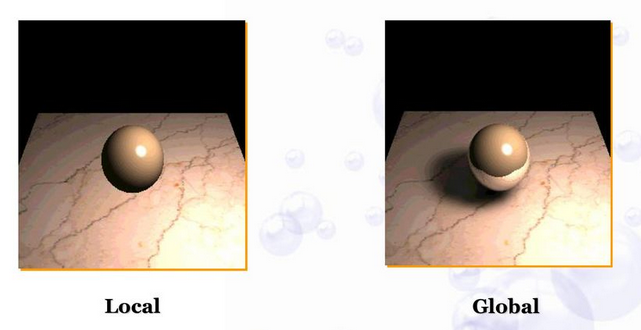
\includegraphics[width=\linewidth]{assets/local_vs_global}
    \captionof{figure}{Dibujado utilizando iluminación local y global}
    \label{local-vs-global-img}
\end{minipage}

\subsection{Iluminación Local}
\label{sec:ilumlocal}
Los modelos de iluminación local como el propuesto por \citeauthor{Phong} en \citeyear{Phong} tienen en cuenta las propiedades físicas de los materiales
y las superficies de cada uno de los objetos de la escena de forma individual. Es decir, al dibujar uno de los
objetos no se toman en cuenta las posibles interacciones de los haces de luz con los objetos restantes.

En referencia a la ecuación del rendering, el término
geométrico nunca toma el valor 0 es decir, no se toma en cuenta las colisiones de los haces de luz con otros
objetos, $\epsilon(x,x')$ toma un valor constante (independiente de $x'$) y $\int_{S} \rho(x,x',x'')I(x',x'') \delta x''$ toma el valor constante $1$.

\subsection{Iluminación Global}
\label{sec:ilumglobal}

El término iluminación global refiere a una modelo de
computación gráfica que simula completamente las interacciones de la luz con todos los objetos que se encuentran 
en la escena. Es decir, en contraposición a la iluminación local, se consideran los fenómenos de
reflexión y refracción de la luz.

\section{Radiosidad}
\label{sec:radiosidad}

El transporte de la luz entre superficies puede ser modelado a través de la propiedad física conocida como
la radiosidad, definida como el flujo de energía irradiada por unidad de área. 

Originalmente, este modelo de iluminación global fue propuesto por \citeauthor{Goral} en \citeyear{Goral} se basa en modelos matemáticos
similares a los que resuelven el problema de la transferencia de calor en sistemas cerrados, conocidos como métodos de elementos finitos.

\subsection{Radiosidad en superficies lambertianas}

La solución propuesta por \citeauthor{Goral} implica que todas las superficies son idealmente lambertianas. Además considerara
que cada superficie irradia energía lumínica en todas direcciones en un diferencial de área $\delta_{A}$, para una dirección de vista $\omega$ puede ser definida como:

\begin{equation}
    i = \frac{\delta{P}}{\cos{\phi\delta\omega}} \label{eq:i}
\end{equation}
donde:
\begin{itemize}
    \item $i$ es la intensidad de la radiación para un punto de vista particular
    \item $\delta{P}$ es lae energía de la radiación que hemana la superficie en al dirección $\phi$ con ángulo sólido $\delta\omega$
\end{itemize}

En superficies perfectamente lambertianas, la energía reflejada puede ser expresada como: $\frac{\delta{P}}{\delta{\omega}} = k\cos{\phi}$. Donde $k$ es una constante.
Sustituyendo en \eqref{eq:i} se obtiene: $\frac{\delta{P}}{\delta{\omega}} = \frac{k\cos{\phi}}{\cos{\phi}} = k$, esto implica que la energía percibida de un punto $x$ 
es constante, independientemente del punto de vista.

Es por esto que la energía total que deja una superficie ($P$) puede ser calculada integrando la energía que deja la superficie en cada dirección posible,
esto es, se integra la energía saliente en un hemiesfera centrada en el punto estudiado:

\begin{equation}
    P = \int_{2\pi} \delta{P} = \int_{2\pi} i\cos{\phi}\delta{\omega} = i \int_{2\pi} \cos{\phi}\delta{\omega} = i\pi \label{eq:P}
\end{equation}

Por tanto, dada una superficie $S_{i}$, es posible calcular la energía lumínica que deja la superficie utilizando \eqref{eq:P}.
Resta definir la \textit{cerradura} de una superficie, definiremos la cerradura de una superficie como los límites que definen los puntos internos y externos de esta, llamaremos parche a cada una de estas superficies cerradas. Esto hace que el problema sea resoluble utilizando métodos de elementos finitos, con esta re-formulación 
del problema, es fácilmente trasladable a la ecuación \eqref{eq:rendering}.

\begin{equation}
    B_{j} = E_{j} + \rho_{j} \sum_{i=1}{N} B_{i} F_{ij} \label{eq:radiosity}
\end{equation}
donde:
\begin{itemize}
    \item $B_{j}$ es la intensidad lumínica (radiosidad) que deja la superficie $j$.
    \item $E_{j}$ es la intensidad lumínica directamente emitida por $j$.
    \item $\rho_{j}$ es la reflectividad del material para la superficie $j$.
    \item $F_{ij}$ se denomina \textit{factor de forma}, un término que representa la fracción de energía lumínica
    que deja la superficie $i$ y llega a $j$. 
\end{itemize}

Cabe destacar que la naturaleza recursiva de la ecuación anterior, implica que se toman en cuenta todas las reflexiones 
difusas que existan en la escena. Como puede observarse, resolver el sistema de $N$ ecuaciones lineales 
bastaría para conocer la energía emitida por cada superficie cerrada. 

$E$, $\mathbf{\rho}$ dependen de los materiales que compongan la escena, son parámetros dados. Sin embargo, 
resta computar la matriz de factores de forma $\mathbf{F}$ para finalmente obtener el vector de radiosidades $B$. 
Para determinar una entrada de la matriz $F_{ij}$ involucrando a las superficies $i$ y $j$ de área $A(i)$, $A(j)$,
considerando los diferenciales infinitesimales de área $\delta{A_{i}}$, $\delta{A_{j}}$ el ángulo sólido visto por
$\delta{A_{i}}$ es $\delta{\omega} = \frac{\cos{\phi_{j}\delta{A_{j}}}}{r^{2}}$. Sustituyendo en \eqref{eq:P} se obtiene:

\begin{equation}
    \delta{P}_{i}\delta{A_{i}} = i_{i} \cos{\phi_{i}}\delta{\omega}\delta{A_{i}} = \frac{P_{i}\cos{\phi_{i}}\cos{\phi_{j}}\delta{A_{i}}\delta{A_{j}}}{\pi r^{2}}
\end{equation}

Considerando que ${P}_{i}{A_{i}}$ es la energía que deja $i$, y que el factor de forma $F_{ij}$ representa el porcentaje
de dicha energía que llega a $j$ podemos observar que:

\begin{equation}
    F_{\delta{A_{i}}-\delta{A_{j}}} = \frac{\frac{P_{i}\cos{\phi_{i}}\cos{\phi_{j}}\delta{A_{i}}\delta{A_{j}}}{\pi r^{2}}}{P_{i}\delta{A_{i}}} = \frac{\cos{\phi_{i}}\cos{\phi_{j}}\delta{A_{i}}}{\pi{r^{2}}}
\end{equation}

Integrando, para obtener el factor de forma para el área total:

\begin{equation}
    F_{ij} = \frac{1}{A_{i}} \int_{A_{i}}\int_{A_{j}}\frac{\cos{\phi_{i}}\cos{\phi_{j}}\delta{A_{i}}\delta{A_{j}}}{\pi{r^{2}}} \label{eq:ff}    
\end{equation}

De \eqref{eq:ff} se obtienen las siguientes propiedades:
\begin{enumerate}
	\label{propsff}
    \item $A_{i}F_{ij} = A_{j}F{ji}$
    \item $\sum_{j=1}^{N} F_{ij} = 1$
    \item $F_{ii} = 0$
    \item $F_{ij}$ toma el valor correspondiente a la proyección de $j$ en una hemiesfera unitaria centrada en $i$, proyectándola a su vez en un disco unitario.
\end{enumerate}

\section{Métodos de cálculo de la matriz de Factores de Forma}
\label{sec:calculoff}

El cálculo de la matriz de factores de forma $\mathbf{F}$ supone la proyección de los parches, de aquí en más se podrá asumir que estos parches son polígonos y por tanto es posible utilizar las técnicas de dibujado de objetos tridimensionales tradicionales.

\subsection{Rasterización}

La <<tubería de renderizado>> es un proceso de dibujado estándar que consiste en un conjunto de etapas bien definidas. Los fabricantes de los dispositivos aceleradores proveen de interfaces de programación (OpenGL, Vuljan, DirectX) que se basan en este modelo para abstraer el uso del hardware.

Si bien la <<tubería de renderizado>> es sumamente modificable por el programador, cada uno de estas etapas cuentan con pequeñas funciones, también llamadas \textit{kernels} o\textit{shaders} que son ejecutadas en la GPU y transforman los parámetros de la entrada en parámetros que recibirá la siguiente. A continuación, se describe el proceso para OpenGL 4.5 \cite{OpenGLWiki}, aunque muchas de estas etapas son trasladables a otras tecnologías.

\begin{enumerate}
	\item Procesamiento de primitivas geométricas:
		Inicialmente, las aplicaciones indican un conjunto de vértices a dibujar, definiendo cierto conjunto de primitivas geométricas como triángulos, cuadriláteros, puntos, líneas u otros. Luego, se procede al procesamiento de estos vértices:
		\begin{enumerate}
			\item Vertex shader: Esta etapa convierte los vértices de entrada suministrados por la aplicación, generalmente se realizan las transformaciones necesarias para transformar el sistema de coordenadas del objeto a un sistema global. Las coordenadas retornadas deberán corresponderse con coordenadas del espacio de recorte. Es decir, coordenadas correspondientes al frustum de vista.
			\item Geometry shader: En esta etapa se procesan los vértices a nivel de primitiva geométrica, es decir, se recibe como parámetro una primitiva geométrica que se transforma en cero o más dependiendo de los parámetros deseados.
			\item Recortado: Esta etapa es \textit{fija}, es decir, no es programable. Todas las primitivas calculadas anteriormente que residan fuera del frustum serán descartadas en las etapas futuras. Además, se transforma las primitivas a coordenadas de espacio de ventana.
			\item Descarte: El proceso de descarte (en inglés \textit{culling}) consiste en la eliminación de primitivas que no cumplan ciertas condiciones, como por ejemplo el descarte de caras cuya normal tiene dirección opuesta a la del observador.
		\end{enumerate}
	\item Procesamiento de fragmentos (rasterización):
		El proceso de rasterización genera un conjunto de fragmentos, que se corresponden con los píxeles finales del resultado.
		\begin{enumerate}
			\item Fragment shader: El procesamiento de cada fragmento se realiza a través del \textit{fragment shader} que calcula uno o más colores, un valor de profundidad, y valores de planilla (del inglés \textit{plantilla}).
			\item Scissor test: Todos los fragmentos fuera de un área rectangular definida por la aplicación son descartados.
			\item Stencil test: Los fragmentos que no pasan la función de planilla definida por la aplicación no son dibujados, por ejemplo, simular el \textit{scissor test} que requieran primitivas más complejas.
			\item Depth test: En esta etapa se ejecuta el algoritmo del Z-Buffer, donde sólo se escribirá el resultado de aquellos fragmentos que tengan la menor profundidad. Es decir, los que se encuentren más cerca del observador.
		\end{enumerate}
\end{enumerate}

Esta técnica de dibujado es extremadamente rápida, además la mayoría de dispositivos contienen hardware especializado capaz de acelerar estos cálculos, comúnmente conocidos como Unidades de Procesamiento Gráfico (o GPU en sus siglas en inglés). Con el objetivo de aprovechar este hardware \citeauthor{Cohen} idearon el método del hemicubo para el cálculo de factores de forma.

\subsubsection{El método del hemicubo}

El hardware optimizado para realizar operaciones de rasterización tiene la capacidad de proyectar escenas tridimensionales en imágenes bidimencionales a gran velocidad.

Para utilizar el hardware eficientemente consideraremos que se calculará una fila completa de $\mathbf{F}$, esto implica que dada $S_{i]}$, una superficie, calcularemos simultáneamente los factores de forma para las superficies restantes. 

El método original propone la proyección de la escena una hemiesfera centrada en $S_{i}$, sin embargo los modelos de proyección utilizados no lo permiten. Por esto es necesario proyectar la escena a un hemicubo centrado en $S_{i}$, esto supone el dibujado de cinco superficies bidimensionales, y por tanto puede ser realizada utilizando la rasterización.

Este método aprovecha el buffer de profundidad (Z-buffer), tomando en cuenta los píxeles proyectados para los elementos que se encuentren más cercanos al parche $S_{i}$.

El algoritmo, propuesto originalmente por \citeauthor{Cohen} en \citeyear{Cohen}, propone rasterizar la escena tridimencional en cinco texturas correspondientes al hemicubo, para cada pixel renderizado se sumará un valor diferencial del factor de forma, que dependerá de la posición del píxel en el hemicubo en relación a la hemiesfera que este aproxima. Esta suma genera una fila de la matriz $\mathbf{F}$, específicamente la fila $\mathbf{F}_{i}$.

Por tanto, podremos definir:

\begin{equation}
	\mathbf{F}_{ij} = \sum_{q=1}^{R} \delta{F_{q}}
	\label{eq:ffgreenberg}
\end{equation}
donde:
\begin{itemize}
	\item $R$ es la cantidad de píxeles correspondientes a la superficie $S_{j}$ que cubren el hemicubo.
	\item $\delta{F_{q}}$ el diferencial de factor de forma asociado al píxel del hemicubo $q$.
\end{itemize}

Los diferenciales de factores de forma deben corregir la deformación introducida con el cambio de proyección desde una hemiesfera a un hemicubo, para ello, para cada píxel que compone el hemicubo es necesario calcular la proporición de área que este término ocupa en la hemiesfera unitaria.

Para la cara superior, los diferenciales se calculan como:

\begin{equation}
	\delta{F_{q}} = \frac{\cos{\phi_{i}}\cos{\phi_{j}}}{\pi{r^{2}}} \delta{A} = \frac{\delta{A}}{\pi({x^{2} + y^{2} + 1})} 
\end{equation}

Para las caras laterales, la fórmula dada es:

\begin{equation}
\delta{F_{q}} = \frac{\cos{\phi_{i}}\cos{\phi_{j}}}{\pi{r^{2}}}\delta{A} = \frac{z\delta{A}}{\pi({x^{2} + z^{2} + 1})}
\end{equation}


\subsection{Trazado de rayos}
\label{sec:raytracing}

Otra de las técnicas de emulación de iluminación existente es el trazado de rayos, consiste en la computación de los puntos de intersección de una semi-recta (a la que denominaremos rayo) con la geometría de la escena, cada uno de estos rayos emulará el transporte de los haces de luz emitidos.

Para cada uno de los rayos emitidos, se determinará el punto de intersección más cercano, luego es posible establecer qué primitiva geométrica fue interceptada y por tanto es posible deducir distintos valores dependiendo del problema en cuestión.

El trazado de rayos es una técnica efectiva \cite{Kajiya} para computar la ecuación del rendering, utilizando la técnica de trazado de camino donde el haz de luz absorbe las propiedades de los materiales con los que interacciona. Por tanto, cada uno de los rayos observados computa uno de los integrandos de la ecuación.

\section{Cálculo del vector de radiosidades}

Luego de computar la matriz $\mathbf{F}$ y dado los vectores de emisiones $E$ y reflexiones $\rho$, resta computar el vector de radiosidades correspondiente para cada parche, denominado $B$.

Recordando \eqref{eq:radiosity}, es posible deducir el problema al sistema de ecuaciones dado por:

\begin{equation}
	E = (\mathbf{I} - \mathbf{RF})B
\end{equation}

Los estudios de álgebra lineal modernos permiten la resolución de sistemas de ecuaciones de forma optimizada, dependiendo de las propiedades observadas.

Recordando las propiedades en \ref{propsff}, podemos observar que:

\begin{itemize}
	\item $\sum_{j=1}^{N} \mathbf{F}_{ij} \leq 1 \forall{i \in [1,N]}$
	\item $\rho_{i} \leq 1 \rightarrow \sum_{j=1}^{N} \mathbf{R}_{ij} \leq 1 \forall{i \in [1,N]}$
\end{itemize}

Esto implica que las entradas de $\mathbf{RF}$ son siempre menores a $1$, por tanto, $(\mathbf{I} - \mathbf{RF}) = M$ es diagonal dominante ya que $\sum_{j=1}^{N}|R_{ij}F_{ij}| \le 1 \forall i \in [1, N]$ y $R_{ii}F_{ii} = 0  \forall i \in [1,N]$. Esto garantiza la convergencia del uso de métodos de resolución iterativos, como el algoritmo de Gauss-Seidel.

Si bien existen maneras alternativas de resolución del sistema planteado con consideraciones específicas del problema a efectos de esta investigación se considerarán los métodos de resolución de ecuaciones lineales que requieran a lo sumo esta propiedad.

Cabe aclarar, que el método planteado hasta el momento resuelve la radiosidad en un único canal. Es decir, no se toma en cuenta todo el espectro electromagnético de la luz, es por ello que puede establecerse una extensión del método. Esta extensión implica la existencia de tres vectores de reflexión, uno para cada canal \textit{RGB}. Por tanto es necesario que se resuelvan tres y no un único sistema de ecuaciones, aunque cabe destacar que la matriz $\mathbf{F}$ permanece constante, ya que las oclusiones geométricas no dependen de la longitud de onda.